
\section{Esercizio 3.1.1}
\subsection{Problem Statement}

Considera la matrice
\[
A = \begin{pmatrix}
4 & -i & 2 \\
i & 2 & 2 + 7i \\
2 & 2 - 7i & -2
\end{pmatrix}
\]

\begin{enumerate}
    \item Calcola l'autovalore massimo e il corrispondente autovettore utilizzando il \textit{Power Method}. Introduci un criterio di arresto basato su una data tolleranza sull'autovalore, ad esempio $10^{-6}$, o basato su un numero massimo di iterazioni. Verifica la correttezza dell'algoritmo.
    
    \item Calcola l'autovalore minimo con il \textit{Inverse Power Method} utilizzando il risolutore QR sviluppato negli esercizi precedenti.
    
    \item Studia numericamente la convergenza degli algoritmi. Definisci $\lambda_1^n$ come l'autovalore massimo ottenuto dal \textit{Power Method} dopo $n$ iterazioni e $\lambda_3^n$ come l'autovalore minimo ottenuto dall'\textit{Inverse Power Method}. Successivamente, rappresenta graficamente $|\lambda_1^n / \lambda_1 - 1|$ e $|\lambda_3^n / \lambda_3 - 1|$ in funzione delle iterazioni.
\end{enumerate}

\subsection{Premessa Teorica}
Il \textit{Power Method} (\textit{PM}) è uno degli algoritmi più semplici per estrarre gli autovalori di una generica matrice $A \in \mathbb{C}^{N \times N}$ diagonalizzabile e con un autovalore dominante in modulo, in particolare, il metodo restituisce una stima dell'autovalore di modulo maggiore. È possibile definire un \textit{Inverse Power Method} (\textit{IPM}) che determini l'autovalore minimo della matrice. Questi vengono definiti algoritmi iterativi, cioè che determinano il risultato con uno specifico grado di precisione, ma non convergono in un numero finito di passaggi al valore vero. Nel corso della discussione dei metodi presenentiamo il caso di matrice reale per semplicità: il passaggio ad una complessa richiede di sostituire $A^T \longrightarrow A^\dagger$.

\subsection{Metodi Numerici e Algoritmi}
\subsubsection{Power Method}
Data $A^{N\times N}$ e scegliendo un generico vettore di partenza $\boldsymbol{x_0}$, possiamo definire:
\[
\boldsymbol{y}(n) = A^n \boldsymbol x_0 = \dots = \lambda_1^n \left[ c_1 \boldsymbol{v}_1 + \sum_{i=2}^{N} c_i \left( \frac{\lambda_i}{\lambda_1} \right)^n \boldsymbol{v}_i \right], \quad \quad \left| \frac{\lambda_i}{\lambda_1} \right| < 1
\]
quindi, grazie all'ultima riscrittura, prendendo il limite per $n \xrightarrow{} \infty$, cioè per un grande numero di iterazioni dell'algoritmo:
\begin{equation} \label{eq: Direct Method autovett}
\lim_{n \xrightarrow{}\infty} \boldsymbol{y}(n) = c_1 \lambda_1^n \boldsymbol{v}_1
\end{equation}
L'ultimo risultato ci porta a determinare univocamente, a meno della normalizzazione, l'autovettore associato a $\lambda_1$. La soluzione è non banale se e solo se il vettore iniziale $\boldsymbol x_0$ non è ortogonale
\footnote{
Ci occupiamo di questa eventualità semplicemente definenedo il vettore $\boldsymbol x_0$ con direzione casuale.
}
a $\boldsymbol{v}_1$, poichè quello che l'algoritmo fa è applicare la matrice al vettore generico, ridirezionandolo e riscalandolo:
\begin{enumerate}
    \item Con la normalizzazione ad ogni step eliminiamo il \textit{rescaling} ($y \longrightarrow \frac{y}{||y||}$).
    \item Iterando per un numero di volte sufficientemente grande vediamo che il contributo principale è quello dell'autovalore maggiore, quindi ci aspettiamo che il vettore finale sia sovrapponibile all'autovettore associato a $\lambda_1$ (cfr. Eq.~\eqref{eq: Direct Method autovett}).
\end{enumerate}
Alla definizione dell'autovettore possiamo infine discutere quella dell'autovalore, usando il "Coefficiente di Rayleigh" come segue:
\begin{equation} \label{eq: Rayleigh Coeff}
\lim_{n\to\infty} \lambda_1^{(n)} = \lim_{n\to\infty} \frac{\boldsymbol{y}(n)^T A \boldsymbol{y}(n)}{\boldsymbol{y}(n)^T \boldsymbol{y}(n)} = \lambda_1
\end{equation}

\noindent Per ottimizzare l'algoritmo definiamo $\boldsymbol y = A\boldsymbol x_0$, successivamente calcoliamo per ogni iterazione\\ $\boldsymbol y(k+1) = A\boldsymbol y(k)$: quando terminiamo l'algoritmo, dopo un numero $n$ di iterazioni, il valore di $\boldsymbol y(n) = A^n \boldsymbol x_0$.\\

\noindent Si può dimostrare che il \textit{Power Method} così definito ha convergenza lineare.

\subsubsection{Inverse Power method} \label{sec: Inverse Pow mth}
Analizzando la matrice inversa di $A$ possiamo dire che essa avrà gli stessi autovettori dell'originale, ma le corrisponderanno autovalori inversi, cioè:
\[
A\boldsymbol v_1 =\lambda_1 \boldsymbol v_1 \xrightarrow{Inversa} A^{-1}\boldsymbol v_1 = \frac{1}{\lambda_1} \boldsymbol v_1
\]
Questo comporta che l'autovalore più piccolo di A diventa il più grande per la sua inversa, possiamo quindi applicare il \textit{PM} e definire iterativamente
\[
\boldsymbol	y(n+1) = A^{-1}\boldsymbol y(n)
\]
Valutare l'inversa di una matrice generica è un'operazione costosa, è però possibile riscrivere la relazione come segue, evitando di dover invertire:
\[
A\boldsymbol y(n+1) = \boldsymbol y(n)
\]
decidiamo infine di procedere implementando l'utilizzo degli algoritmi di scomposizione, in particolare scegliamo \textit{QR decomposition}: 
\[
A = QR 
\]
\[
\longrightarrow{} QR\boldsymbol y_{n+1} = \boldsymbol y_n
\]
\[
\longrightarrow{}R\boldsymbol y_{n+1} = Q^{-1} \boldsymbol y_n
\]
Ricordando che per le proprietà della decomposizione QR, $Q^TQ = I \longrightarrow{}Q^{-1} = Q^T$ (cioè $Q$ è ortogonale)
\[
R\boldsymbol y_{n+1} = Q^T \boldsymbol y_n
\]
ridefinendo $\boldsymbol{b} = Q^T \boldsymbol y_n$, quello che rimane è un sistema lineare molto facilmente risolvibile, tramite una semplice \textit{Backward Substitution} (cfr Cap. \ref{sec: Back-Forw Subst})
\[
R\boldsymbol y_{n+1} = \boldsymbol{b}
\]
ancora una volta, per un numero grande di iterazioni, $\boldsymbol y_n = \boldsymbol v_N$, dove $\boldsymbol v_N$ è l'autovettore relativo all'autovalore più piccolo.
\subsubsection{Shifting}
Un'estensione di questo algoritmo è possibile considerando lo \textit{shifting}: scegliendo un valore di riferimento si può spostare lo spettro di $A$ di un certo scalare.\\
Se scelto in maniera oculata, questo può essere un grande vantaggio, per esempio possiamo ridefinire la matrice come $A \xrightarrow[]{}A - \alpha I$, spostando tutti gli autovalori da $\lambda \xrightarrow[]{}\lambda - \alpha$: se scegliamo $\alpha$ vicino ad un generico autovalore $\lambda_k$ di tutti gli $N$ della matrice, l'operazione che abbiamo appena definito rende $\lambda_k$ quello in modulo più piccolo, che avrà dopo lo \textit{shifting}, un valore confrontabile con lo zero, risultando, guardando la matrice inversa, in un autovalore grande, che permette ad $A^{-1}$ di trasformare il vettore generico proprio in $\boldsymbol{v}_k$ (normalizzato) con poche interazioni.\\
Per avere una stima di $\lambda_k$ da usare come $\alpha$, ricorriamo al \textit{Rayleigh Quotient}, cioè utilizzando la migliore stima possibile, ad una certa iterazione, dell'autovalore.\\
\noindent Si può dimostrare che il Metodo del Quoziente di Rayleigh ha convergenza cubica (e che costa $O(N^2)$, grazie all'utilizzo della \textit{Backward Substitution} e della \textit{QR decomposition}).


\subsection{Risultati e Discussione} \label{sec: Controllo autovalori}
Procediamo ad analizzare le soluzioni ai problemi proposti nell'esercizio:
\begin{enumerate}
    \item Tramite implementazione del \textit{PM} risolviamo il problema della ricerca dell'autovalore in modulo maggiore:
    \begin{elegantcode}
A =
[[ 4.+0.j -0.-1.j  2.+0.j]
 [ 0.+1.j  2.+0.j  2.+7.j]
 [ 2.+0.j  2.-7.j -2.+0.j]]

eig_val_MAX = (8.451876899596735+8.881784197001252e-16j)
eig_vect = [0.63491092-0.59342626j 1.18122253+0.91110263j 0.95772132-0.73031907j]
    \end{elegantcode}
    Abbiamo definito che l'algoritmo abbia arresto nel momento in cui $|\lambda_{n+1} - \lambda_n| <\varepsilon = 10^{-8}$.\\
    Viene valutata la correttezza dei risultati finali in questo modo:
    \begin{elegantcode}
res = A @ eigVect - eigVal * eigVect
err = np.sqrt(np.sum(np.abs(res)**2))
if err > 1e-8:
    raise ValueError("Eigenpair not accurate")
    \end{elegantcode}
    cioè secondo la definizione di autovalore $A \boldsymbol v =\lambda\boldsymbol v$.
    
    \begin{multicols} {2}
        È interessante osservare come l'errore sull'autovalore calcolato, per ogni iterazione, abbia un decadimento esponenziale. In particolare nella Figura \ref{fig: Plot conv Power Mth} rappresentiamo il caso di due matrici $M \in \mathbb{R}^{3\times 3}\ , K \in \mathbb{C}^{3\times 3}$. Per le considerazioni fatte nei paragrafi precedenti ci aspettiamo, in un eventuale confronto, che il \textit{IPM}, a parità di matrice di test, abbia necessità di meno interazioni per arrivare a convergenza.
        
        \begin{figure}[H]
            \centering
            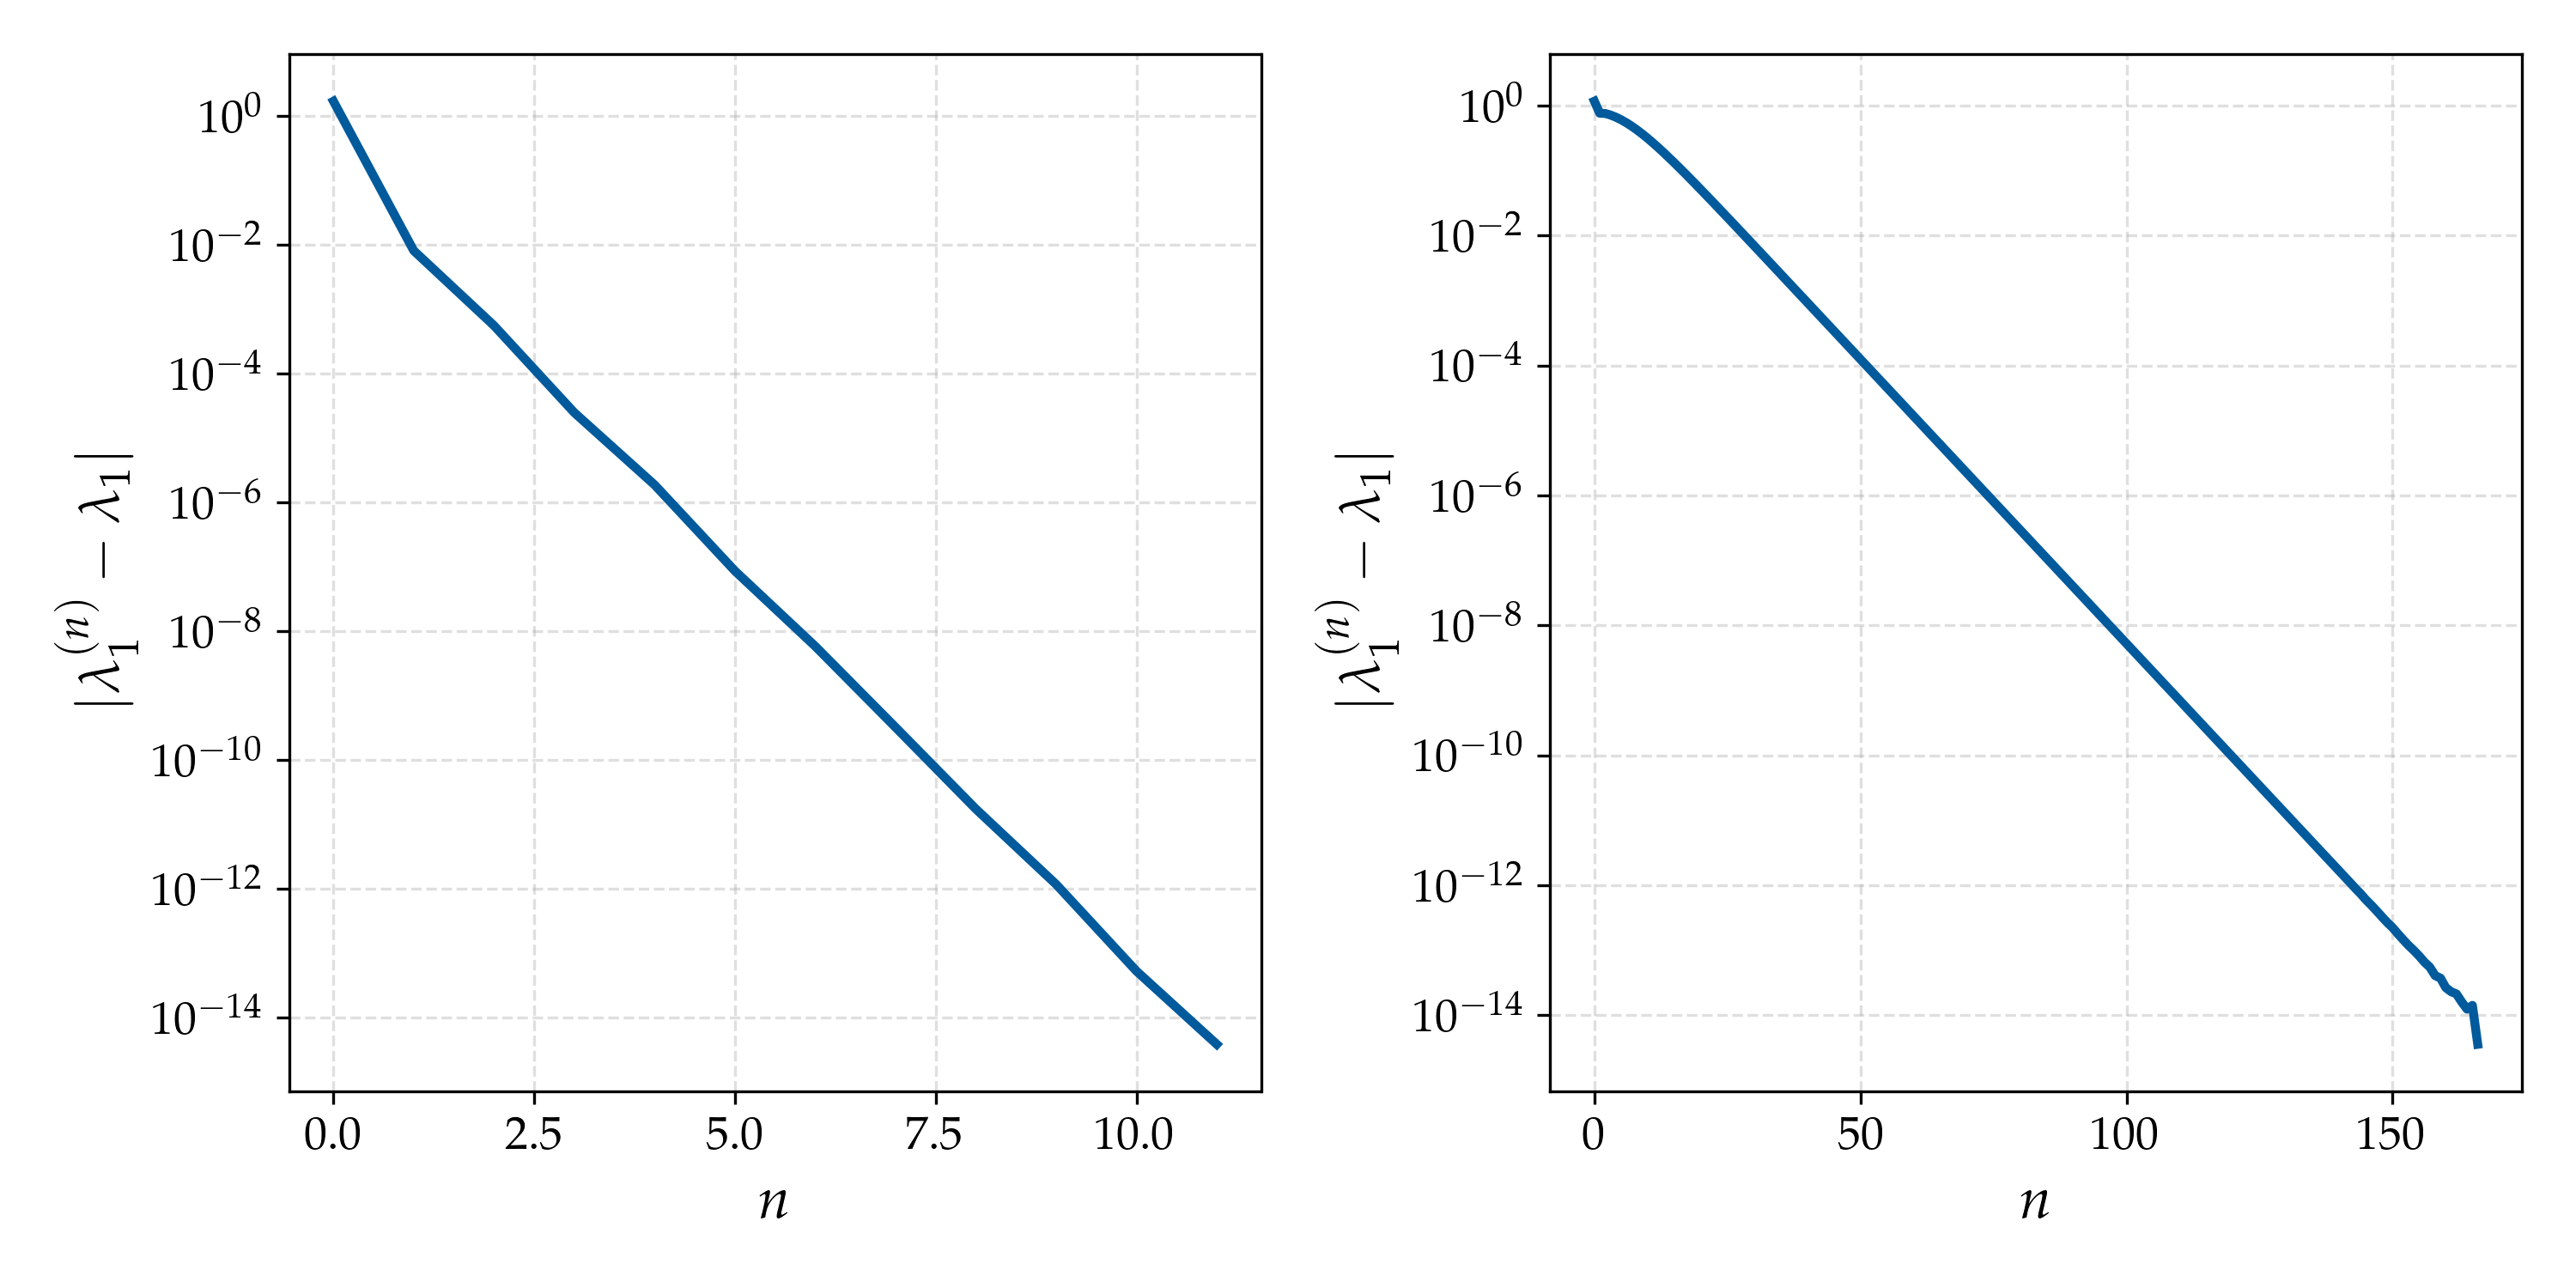
\includegraphics[width=1.1\linewidth]{images/6/plot_powConv.png}
            \caption{Sulla sinistra il caso di $M$, sulla destra $K$. L'andamento della convergenza è lo stesso ma si noti la differenza nel numero di iterazioni necessarie per
            raggiungere la precisione}
            \label{fig: Plot conv Power Mth}
        \end{figure}
    \end{multicols}    

    \item In maniera del tutto simile a quanto fatto in precedenza, e in accordo con ciò che abbiamo descritto nel Cap. \ref{sec: Inverse Pow mth}, risolviamo il problema con questo output:
    \begin{elegantcode}
A =
[[ 4.+0.j -0.-1.j  2.+0.j]
 [ 0.+1.j  2.+0.j  2.+7.j]
 [ 2.+0.j  2.-7.j -2.+0.j]]
 
eig_val_min = (3.1896027470480552-3.51669076861739e-17j)
eig_vect = [ 1.063511 -0.0526563j -0.1124258-0.4313319j -0.2152674-0.0348766j]
    \end{elegantcode}
    
    \item Infine possiamo confrontare i risultati dei due metodi. Gli algoritmi completi sono stati modificati in maniera da restituire la stima dell'autovalore ad ogni step, fino ad un valore fissato di $n=80$ dal quale in poi la precisione dell'\textit{IPM} ha raggiunto la \textit{machine precision} $\varepsilon \approx 10^{-15}$.
    
    
    I valori di confronto per i rapporti ($\lambda_{\text{MAX}}$ e $\lambda_{min}$)sono dati dai punti precedenti dell'esercizio, in cui li abbiamo calcolati esplicitamente. È possibile notare una differenza netta tra la convergenza del primo o del secondo metodo: l'autovalore più piccolo risulta, guardando la matrice inversa, in uno grande, quindi l'effetto dipende dal rapporto tra gli autovalori dell’inversa, cioè $\left|\lambda_{N-1}/\lambda_N\right|$. Ne risulta che l'applicazione della matrice sul vettore random di inizializzazione, ha un effetto più marcato con l'\textit{Inverse}, permettendo una rapida convergenza.

    \begin{figure}[H]
        \centering
        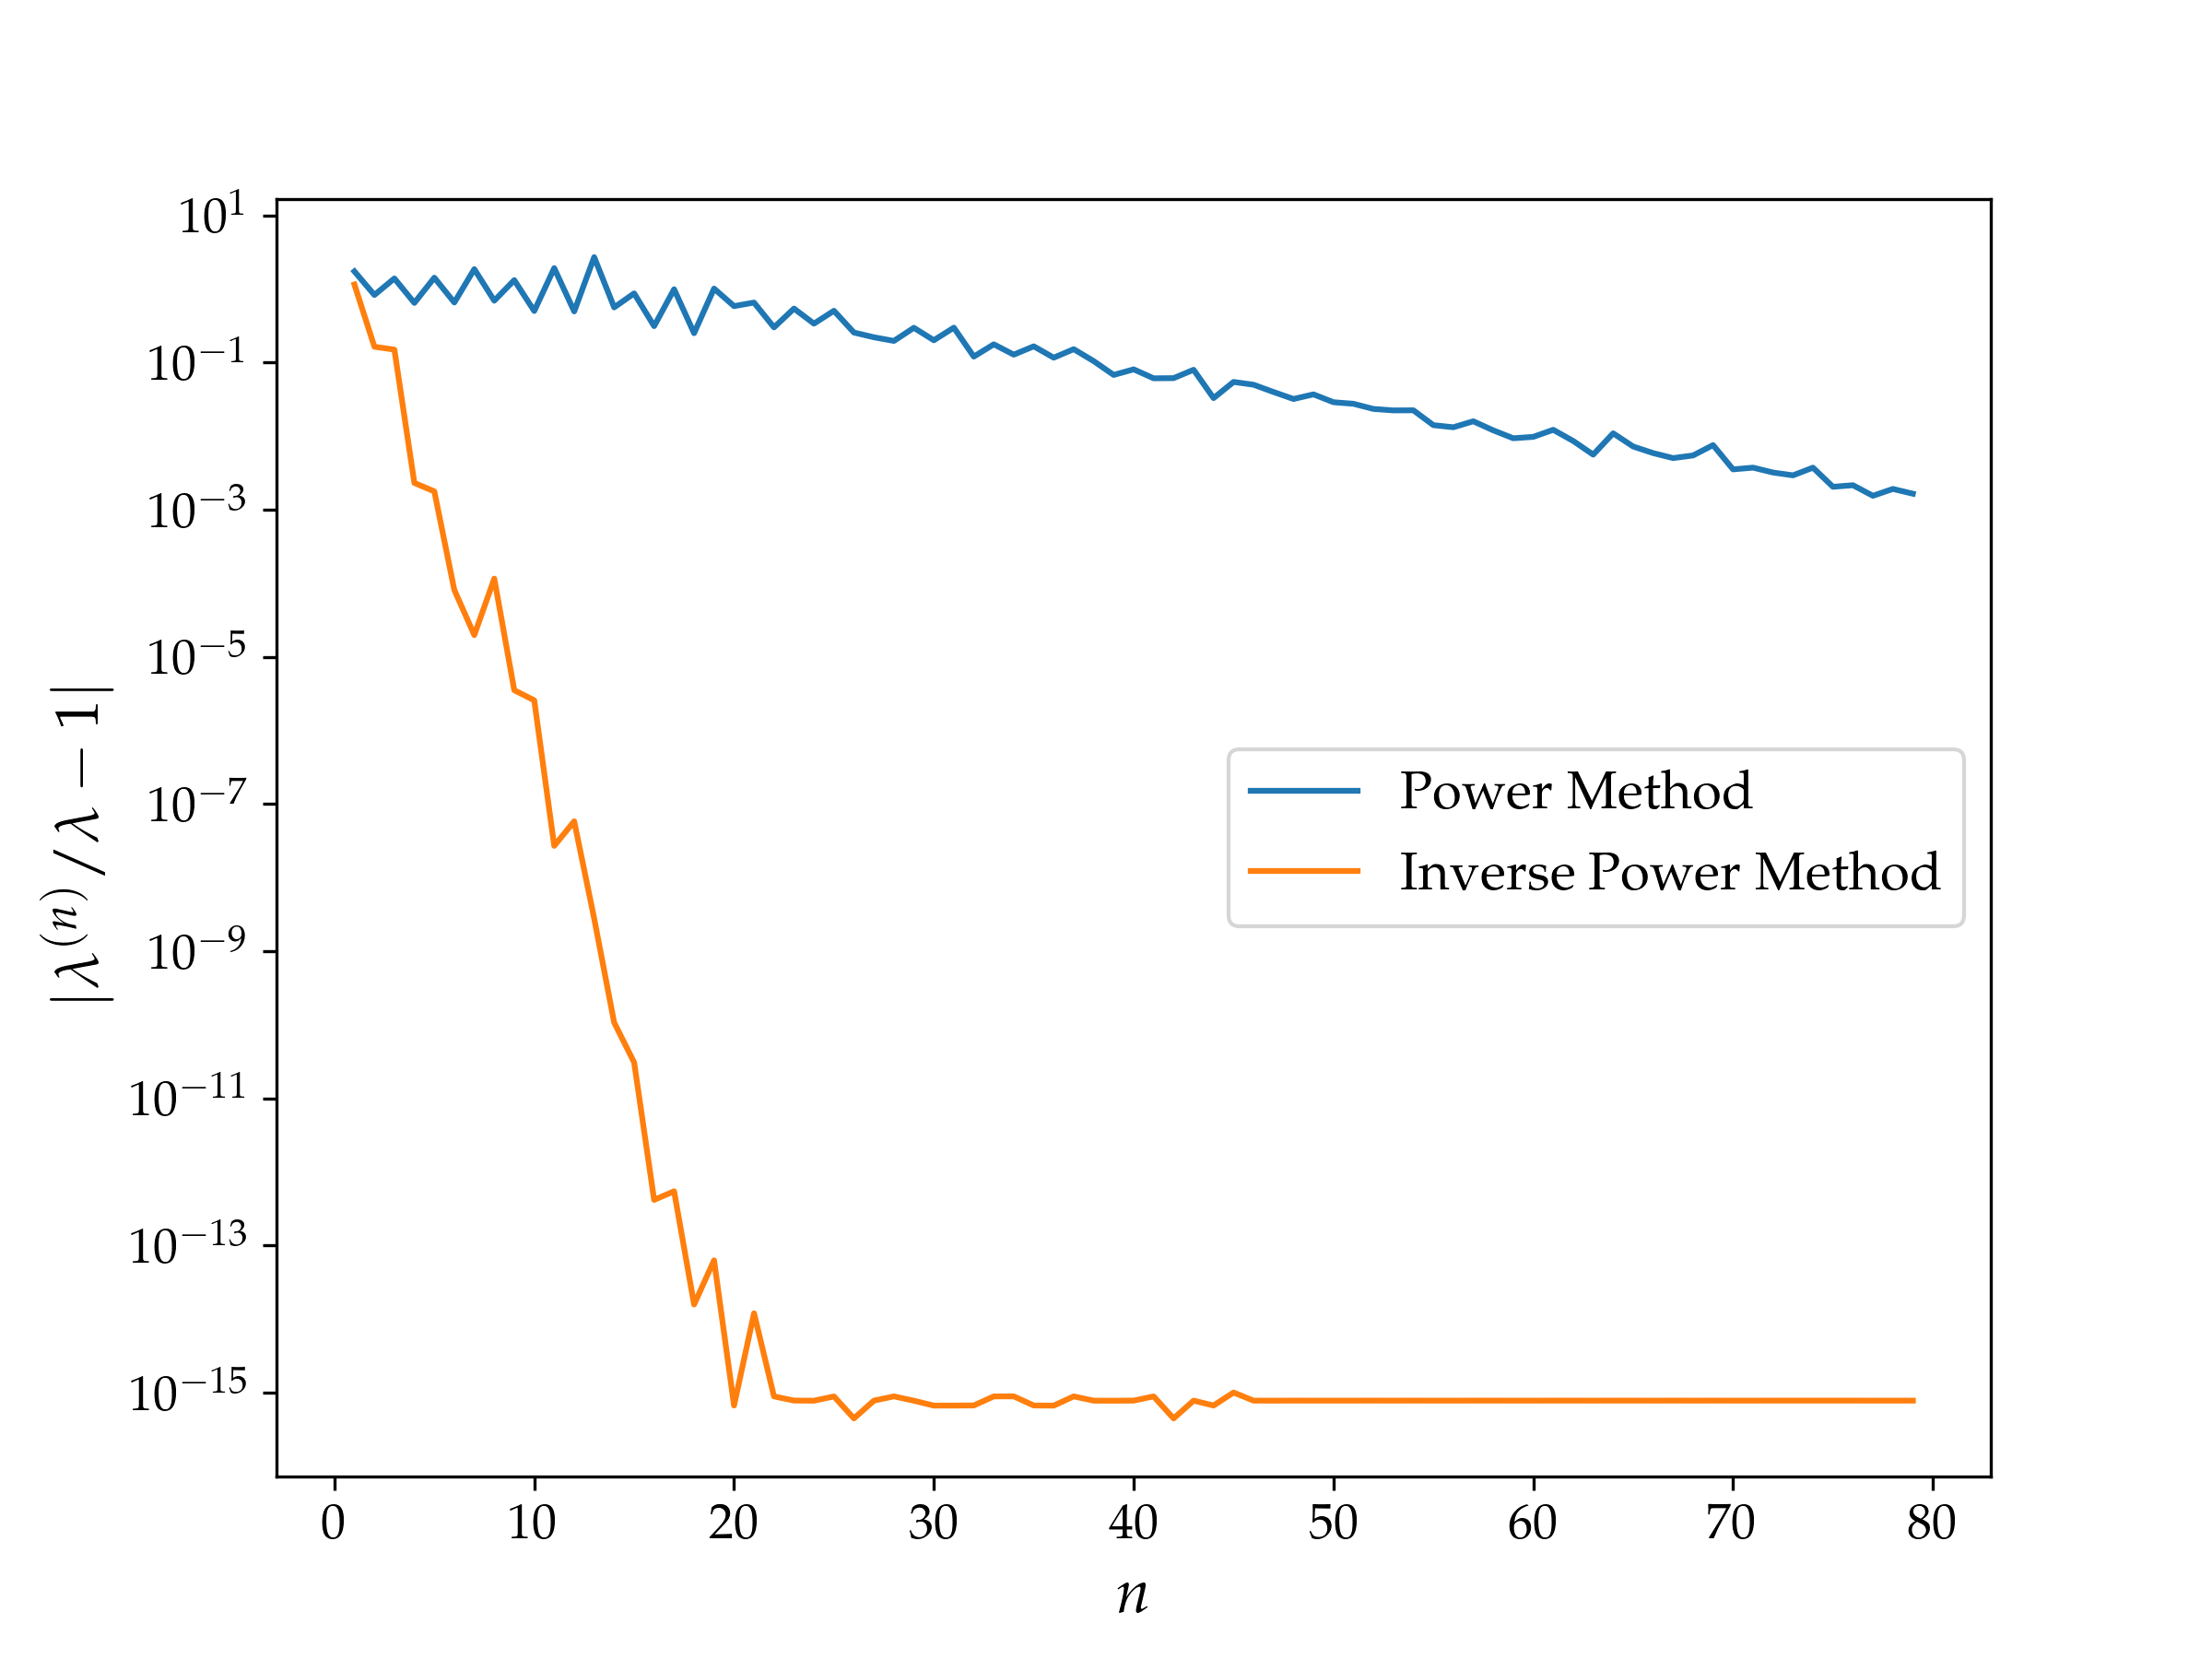
\includegraphics[width=0.7\linewidth]{images/6/pow_vs_inv_convergence.png}
        \caption{Confronto tra il rate di convergenza del \textit{PM} (blu) e quello dell'\textit{IPM} (giallo)}
        \label{fig: Conv Pow vs Inv}
    \end{figure}
\end{enumerate}








\newpage

\section{Esercizio 3.2.1}
\subsection{Problem Statement}
Si implementi una funzione che riceva in ingresso una matrice $A$, una tolleranza $\epsilon$ e un numero massimo di iterazioni $N$. La funzione deve restituire gli autovettori e gli autovalori di $A$ attraverso l'applicazione iterativa della decomposizione $QR$ precedentemente implementata.\\
Poiché si prevede che la matrice risultante $A_\infty$ sia una matrice diagonale (o triangolare superiore a blocchi) contenente gli autovalori lungo la diagonale principale, si definisca un criterio di arresto appropriato. Per testare l'algoritmo, si utilizzi la matrice tridiagonale che rappresenta l'operatore Laplaciano unidimensionale, considerando dimensioni modeste dell'ordine di $O(10)$.\\
Si produca infine un grafico che mostri l'andamento della convergenza per ogni singolo autovalore in funzione del numero di iterazioni.

\subsection{Premessa Teorica}
Una possibilità per lo sviluppo di un algoritmo di estrazione degli autovalori di una matrice sta nei metodi di decomposizione della matrice di test $A$: se è effettivamente possibile implementare un algoritmo che faccia uso della Decomposizione LU, è molto più conveniente lo sviluppo di uno che usi la Decomposizione QR, più stabile e possibile per una qualsiasi matrice generica. Questo rappresenta un metodo di algoritmo iterativo, portandosi dietro tutte le sue potenzialità, ma anche le sue problematiche.

\subsection{Metodi Numerici e Algoritmi}
Si procede definendo iterativamente $A_k$, fissando $A_0 = A$: da qui in poi, potendo decomporre con \textit{QR decomposition}, quindi $A_k = Q_kR_k$, si definisce la matrice al passo $k+1$ come $A_{k+1}=R_kQ_k$. Questa operazione è una trasformazione di similitudine, infatti si può mostrare che $A_{k+1}=Q^\dagger_k A_k Q_k$, e la sua importanza sta nel fatto di conservare lo spettro della matrice originale.\\
Per un numero grande di iterazioni:
\begin{enumerate}
    \item $A_k$ converge verso $A_\infty$, che è la sua diagonalizzata, cioè presenta gli autovalori sulla diagonale e zeri nel resto.
    \item $\prod_{j=0}^k Q_j$, converge a $Q_\infty$, le cui colonne sono gli autovettori che costituiscono una base ortonormale di $A$.
\end{enumerate}
Queste conclusioni sono valide nella maniera qui esposta solo per matrici hermitiane, per una matrice generica $A_\infty$ è triangolare superiore e l'algoritmo si complica. Ci limitiamo quindi a studiare matrici hermitiane, che sono una classe abbastanza rappresentativa per i problemi di fisica che andremo ad analizzare.

\subsection{Risultati e Discussione}
Il test sulla ricerca degli autovalori viene fatto su una matrice $A \in \mathbb{C}^{3 \times 3}$ (hermitiana), definita come segue:
\begin{elegantcode}
ndim = 3
re = np.random.rand(ndim, ndim)
im = np.random.rand(ndim, ndim)
Z = re + 1j * im
A_test = (Z + Z.T.conj()) / 2       # per assicurare A hermitiana
\end{elegantcode}
\noindent L'algoritmo ha il criterio di fermarsi quando smette di vedere una evoluzione nei valori di $A_k$, definito così in codice \textit{.py}

\begin{elegantcode}
if np.sqrt(np.sum(np.abs(Ak - np.diag(np.diag(Ak)))**2)) < tol:
    print(f'Tolerance reached at step {i+1}')
    eigenVal = np.diag(Ak)
    eigenVect = Qk
    return eigenVal, eigenVect
\end{elegantcode}
Il risultato, comprensivo della matrice di test, è espresso nella cella qui sotto:

\begin{elegantcode}
Tolerance reached at step 35

A =
 [[0.56820981+0.j         0.9532166 -0.05799793j 0.47756225-0.09283526j]
 [0.9532166 +0.05799793j 0.30847352+0.j         0.45485252+0.04791834j]
 [0.47756225+0.09283526j 0.45485252-0.04791834j 0.15548257+0.j        ]]

eig_val = [ 1.68903863+1.1017535e-17j -0.53975861-5.9673907e-18j
 -0.11711411+7.2000436e-18j]

eig_vect = [[ 0.68845441-1.24812738e-17j -0.63535769-1.71610507e-02j
  -0.34150506-7.36947240e-02j]
 [ 0.60423579+5.55867258e-02j  0.75235531-2.10953753e-02j
  -0.21152465+1.43467835e-01j]
 [ 0.39534364+3.92829679e-02j -0.05662805+1.62283202e-01j
   0.90091426-3.11635707e-02j]]
\end{elegantcode}
\noindent È possibile verificare che questo risultato è corretto con le stesse modalità espresse nel Cap.\ref{sec: Controllo autovalori}, quindi come segue:
\begin{elegantcode}
if not np.allclose(A_in @ eigenVect, eigenVal * eigenVect, rtol=tol):
    raise ValueError('Eigenpair not accurate')
\end{elegantcode}
\medskip
\noindent Come richiesto dall'esercizio, possiamo svolgere per la matrice tridiagonale che rappresenta il Laplaciano unidimensionale, $K \in \mathbb{Z}^{10\times 10}$, valutando lo spettro.
Diventa molto interessante la figura ottenibile dalla visualizzazione dell'errore in funzione dei singoli autovalori, cioè l'andamento della convergenza per diversi valori di $\lambda$ (Fig. \ref{fig: Conv sing eigen}).

\begin{figure}[H]
    \centering
    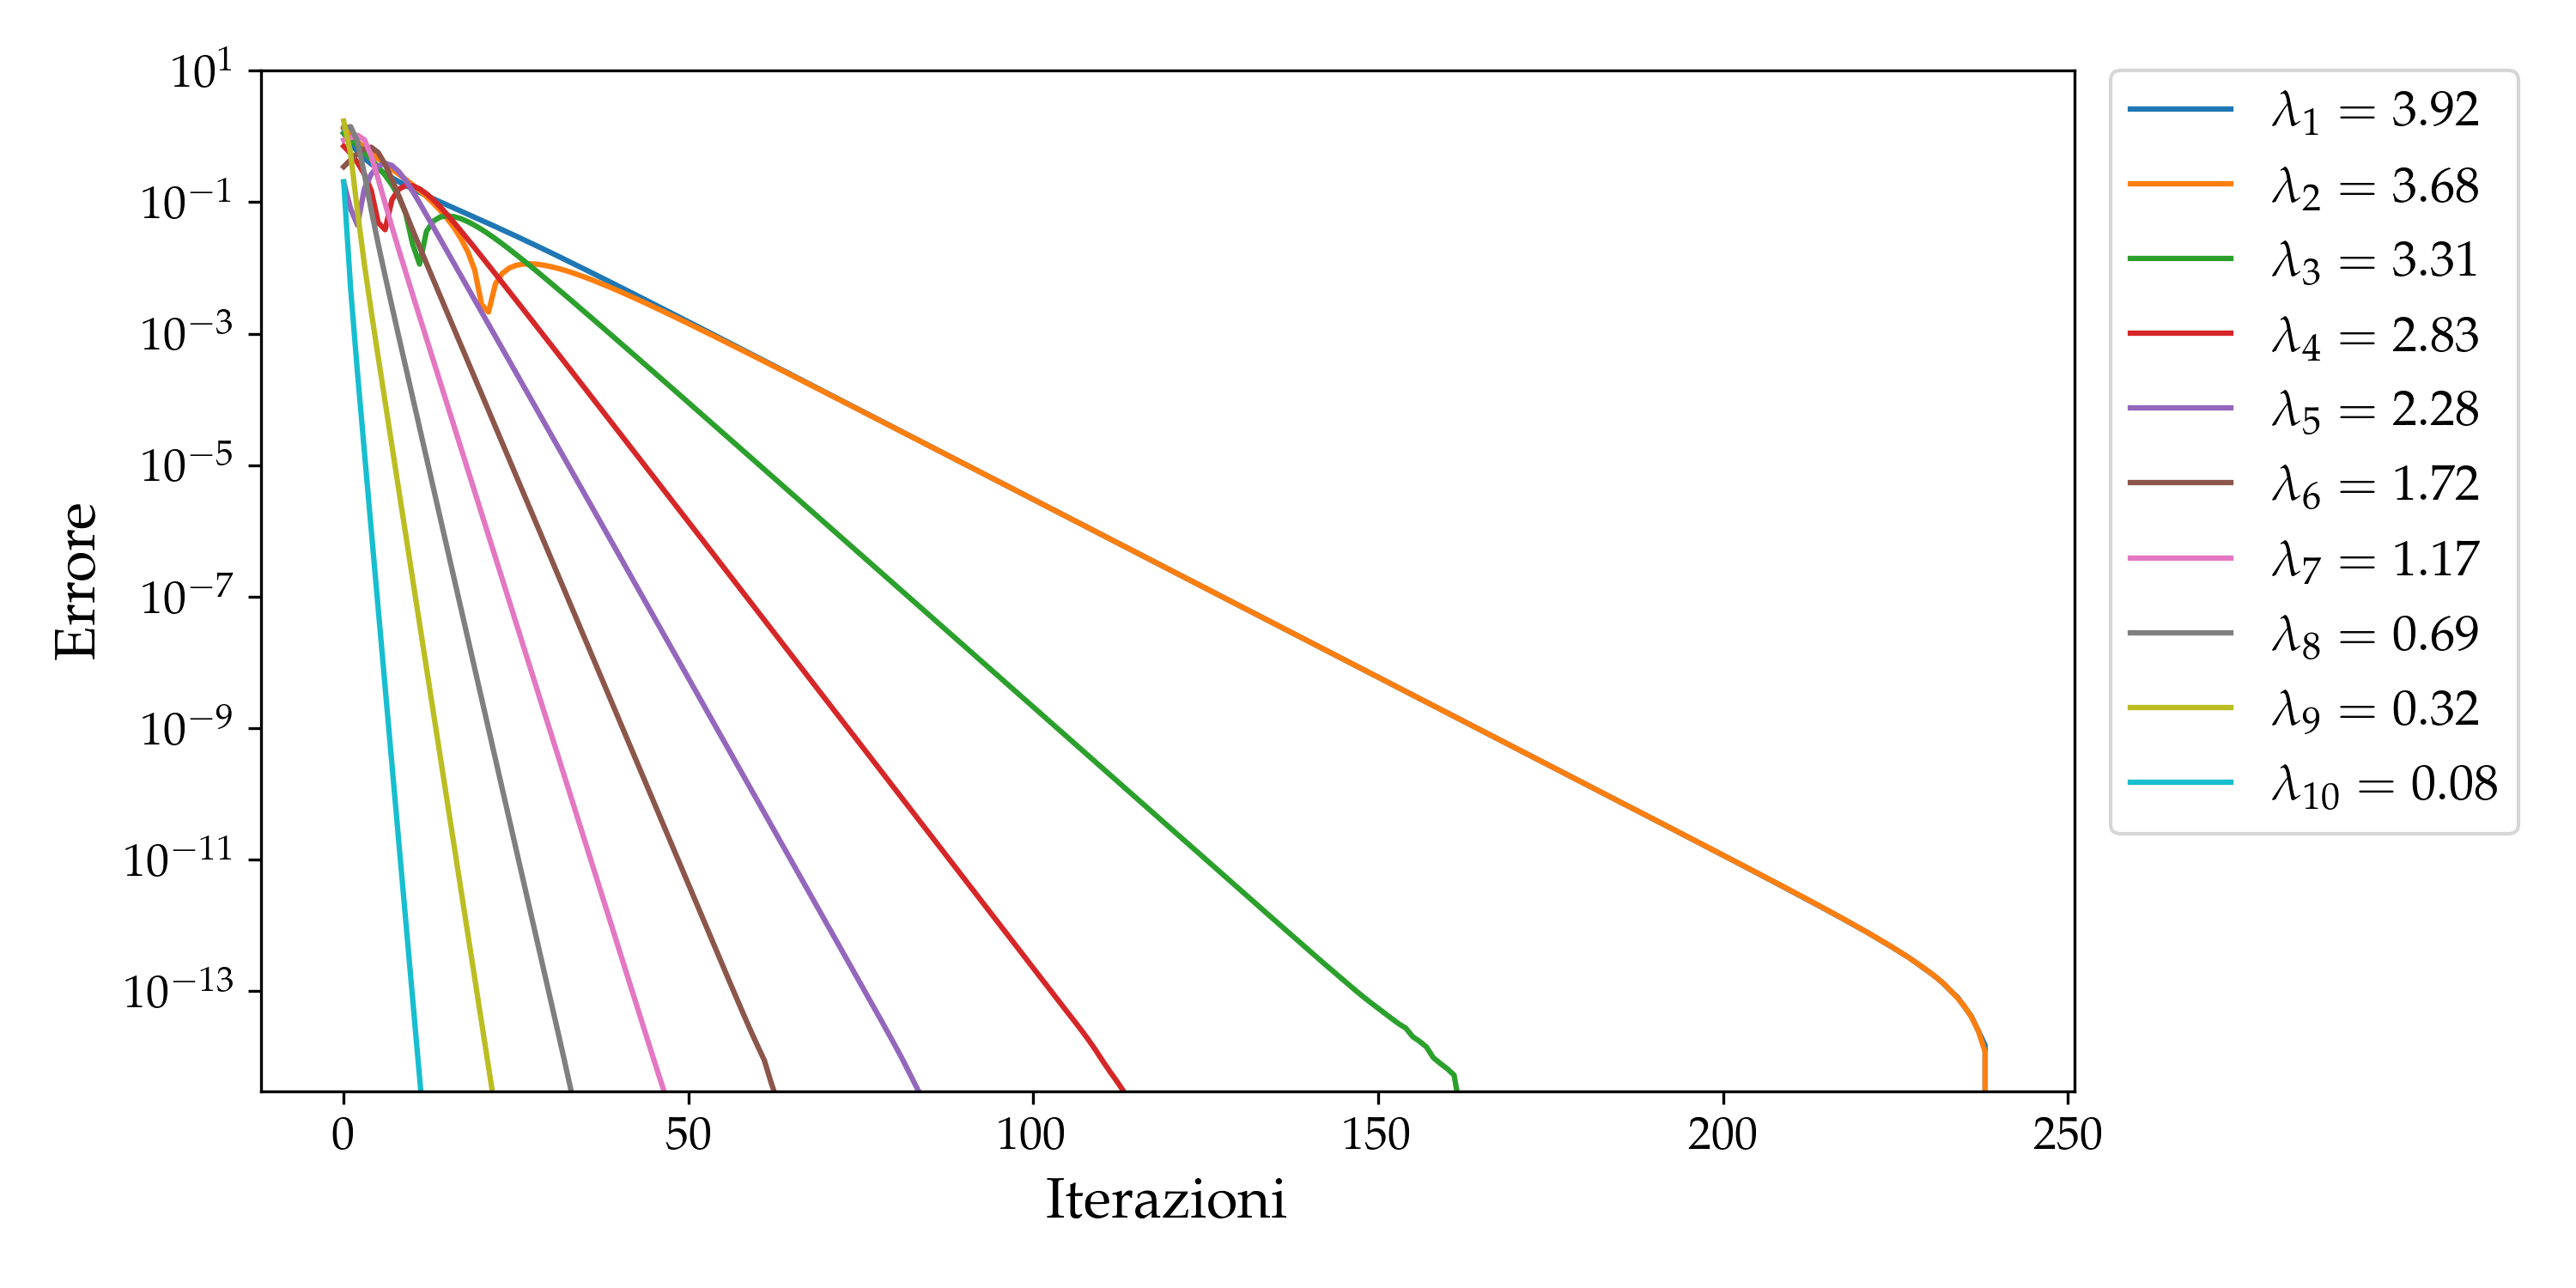
\includegraphics[width=0.7\linewidth]{images/7/conv_single_eigen.png}
    \caption{Andamento della convergenza per diversi autovalori di $K$.}
    \label{fig: Conv sing eigen}
\end{figure}
